\section{Fase di Progettazione}
Come strategie di progettazione abbiamo usato quella del \textit{Mobile First} e \textit{Responsive Web Design}.\\
\textit{Mobile First} permette di caricare gli elementi essenziali sulle piattaforme mobile. Ciò porta un'esperienza di navigazione più snella, che evita ritardi e latenza di caricamento.\\
\textit{Responsive Web design} si basa sul concetto di media query che ottimizzano la visualizzazione in base a dispositivi specifici e dimensioni di viewport.\\
Infatti è stato codificato il CSS iniziale secondo un approccio \textit{Mobile First} e poi utilizzato le media query per servire selettivamente contenuti aggiuntivi al crescere delle dimensioni del viewport.\\
Abbiamo preferito usare XHTML5 perché ci permette di usare la specifica WAI-ARIA descritta nella sezione \ref{subsection:navigazione}.

\subsection{Attori}
Abbiamo individuato tre tipi di attori:
\begin{itemize}
	\item \textbf{Utente non registrato:} può visitare tutti i contenuti del sito in modo ristretto, per esempio non può commentare le pagine. Può registrarsi attraverso un apposito form e diventare un utente registrato;
	\item \textbf{Utente registrato:} è un utente che ha i premessi per scrivere commenti ed eliminare solo i propri, accedere nella propria area riservata avendo la possibilità di creare nuove pagine, modificare ed eliminare solo le proprie;
	\item \textbf{Admin:} è un utente registrato con più permessi di quest'ultimo. Può eliminare utenti, cancellare qualsiasi commento, accettare le pagine pendenti, creare, modificare ed eliminare qualsiasi pagina.
\end{itemize}

\subsubsection{Procedura di modifica e/o inserimento} \label{subsection:modificainserimento}
All'interno di questa piattaforma tutte le modifiche e gli inserimenti devono passare dall'approvazione di un amministratore. Ciò significa che, ogni qualvolta un utente modifica un articolo, tale modifica deve essere memorizzata all'interno della piattaforma. Segue che la piattaforma può ospitare due tipologie di pagine: modificate o meno. Una volta che una di queste modifiche viene approvata dovrà essere eliminata tra quelle proposte e sostituita alla pagina pubblicata corrente, altrimenti, se viene scartata, verrà semplicemente eliminata.
\pagebreak
\subsection{Struttura del sito}
Il sito presenta tre livelli di profondità in modo tale da rendere facile la ricerca manuale senza dover rinunciare ad una organizzazione gerarchica ben strutturata.\\
La struttura della gerarchia del sito è suddivisa in categorie, sottocategorie e infine pagine, ed è così definita:
\begin{itemize}
	\item \textbf{Personaggi:}
	\begin{itemize}
		\item Esseri umani;
		\item Semidivinità/eroi;
		\item Divinità;
		\item Creature.
	\end{itemize}
	\item \textbf{Eventi:}
	\begin{itemize}
		\item Epoca degli dei;
		\item Epoca degli dei e degli uomini;
		\item Epoca degli eroi.
	\end{itemize}
	\item \textbf{Luoghi:}
	\begin{itemize}
		\item Mitologici;
		\item Reali.
	\end{itemize}
\end{itemize}
Le pagine possono essere in due stati differenti:
\begin{itemize}
	\item \textbf{Pendenti:} sono pagine in attesa di approvazione da parte di un amministratore per poter essere pubblicate, non sono visibili sul sito web;
	\item \textbf{Pubblicate:} sono pagine visibili nel sito web.
\end{itemize}

\subsubsection{Header} \label{subsection:header}
All'interno dell'header è presente il \textit{logo} del sito, la \textit{barra di ricerca} e due \textit{pulsanti} che vengono visualizzati in base al tipo di utente (registrato, non registrato) e il \textit{menu}.\\
Il \textit{logo} è situato a sinistra ed è privo di link, infatti il link che rimanda alla homepage è già presente all'interno del menu nella voce Home.\\
La \textit{barra di ricerca} è situata a destra del logo ed orizzontalmente centrato rispetto alla pagina. Questo perché essendo un sito che viene usato principalmente per la ricerca di informazioni riguardanti la mitologia greca, l'utente deve avere subito ciò che vuole, ovvero poter cercare ciò di cui ha bisogno. Grazie al menu a tendina situato alla sinistra del campo di ricerca, l'utente può selezionare la categoria all'interno della quale fare la propria ricerca.\\
Per quanto riguarda la quantità del testo visibile che un utente può scrivere all'interno della barra di ricerca, è stato scelto un numero pari a 30 caratteri. Questo perché un box troppo piccolo aumenta lo stress proporzionalmente per ogni carattere che sfora e gli utenti tendono a scrivere meno con risultati della query più scarsi.\\
Esistono due tipi di \textit{pulsanti} situati a destra della barra di ricerca:
\begin{itemize}
	\item \textbf{Accedi:} viene visualizzato se l'utente non ha effettuato il login al sito;
	\item \textbf{Area Riservata:} viene visualizzato se l'utente ha effettuato il login a sito.
\end{itemize}
Il posizionamento di questi due pulsanti è la stessa anche per la visualizzazione da smartphone, infatti compaiono sulla stessa riga del logo posizionati a destra.\\
Il \textit{menu} compare come left sidebar nella visualizzazione per Desktop, ma fa parte dell'header. Abbiamo scelto questo posizionamento perché, dagli studi fatti sul movimento oculare sugli utenti in una pagina web, si è ricavata una termografia dove le zone calde rappresentano le parti della pagina in cui l'utente ha dedicato più tempo, le quali risultano avere una forma ad F. Di conseguenza avendo il menu a sinistra, l'attenzione ricade su di esso in modo spontaneo.\\

\subsubsection{Breadcrumb}
Il breadcrumb è presente in tutte le pagine del sito, sia mobile che desktop, e comprende un insieme di campi che identificano la posizione dell'utente all'interno del sito. L'ultimo campo è la pagina corrente, ovvero la pagina che l'utente sta visualizzando. Per evitare i link circolari, quest'ultimo campo è solo un testo.

\subsubsection{Contenuto} \label{subsection:contenuto}
Il sito ha lo scopo principale di ricerca e lettura delle informazioni e per questo motivo abbiamo scelto un layout stretto. Infatti, cosi facendo, il numero medio di parole scritte in una riga è di circa 15 e questo permette una migliore lettura.\\
Le informazioni più importanti compaiono nella prima metà della pagina siccome è quella più visibile e che l'utente vede appena viene caricato il sito. Inoltre abbiamo cercato di mettere anche gli elementi fondamentali per l'interazione, come il menu e la barra di ricerca.\\
Lo schema che abbiamo utilizzato è quello a tre panelli, che rispondono alle seguenti domande:
\begin{itemize}
	\item \textbf{Dove sono?:} la prima risposta a questa domanda si trova nel titolo della pagina. Sono brevi e vanno dal particolare al generale. La seconda si trova nei breadcrumb, che indicano il percorso fatto per arrivare in quel punto;
	\item \textbf{Di cosa si tratta?:} la risposta a questa domanda si trova nel contenuto della pagina;
	\item \textbf{Dove posso andare?:} la risposta a questa domanda si trova nel menu che compare come left sidebar.
\end{itemize}

\paragraph{Pagina Home} Questa pagina è la prima che viene visualizzata quando un utente visita il sito. Ha lo scopo di far capire subito all'utente dov'è arrivato e cosa può trovare all'interno del sito.

\paragraph{Pagina Ricerca} A questa pagina ci si arriva dopo aver fatto una ricerca e serve a mostrare i risultati della query fatta dall'utente. Viene mostrata una lista di pagine aventi il nome della pagina e una parte del contenuto di quella pagina. Ogni risultato della query è un link che porta alla pagina corrispondente. 

\paragraph{Pagina Scopri} Questa pagina mostra tutte le categorie e sotto categorie del sito. Una volta che si clicca su una categoria si viene reindirizzati in una pagina che mostra una lista contenente delle pagine random che sono contenute all'interno di quella categoria. Se invece si clicca sulla sotto categoria si viene reindirizzati sulla pagina di Ricerca che mostra la lista di tutte le pagine che sono contenute in quella sotto categoria.

\paragraph{Pagina Contatti} Questa pagina ha lo scopo di dare le informazioni per contattare l'associazione Filo di Arianna oppure di poter mandare una email attraverso il form della pagina.

\paragraph{Pagina Login e Registrazione} Un utente ha la possibilità di registrarsi ed effettuare il login con le sue credenziali. Quando è loggato può accedere alla sua area personale avendo la possibilità di:
\begin{itemize}
	\item \textbf{Creare e modificare pagine:} attraverso una pagina contenente un form dove si inseriscono/modificando le informazioni della pagina;
	\item \textbf{Visualizzare pagine pendenti e pubblicate:} attraverso una pagina che mostra una lista di tutte le pagine pendenti/pubblicate che sono state create da se stesso.
\end{itemize}

\paragraph{Pagina Area Riservata} In questa pagina l'utente può vedere le proprie informazioni personali e, attraverso tre pulsanti, può andare in tre diverse pagine per creare, modificare, visualizzare le pagine create da se stesso. Inoltre l'amministratore visualizza un pulsante in più che porta alla pagina "Gestione degli utenti".

\paragraph{Pagina Articolo e Discussione} Sono due pagine differenti ma vicine l'una all'altra attraverso una visualizzazione a tab. Nella pagina articolo viene mostrato il contenuto dell'articolo, mentre la pagina di discussione mostra tutti i commenti fatti dagli utenti riguardo a quella pagina e si da la possibilità agli utenti loggati di aggiungere dei commenti.

\paragraph{Pagina Gestione utenti} Pagina visualizzabile solo dagli amministratori, la quale permette di eliminare gli utenti registrati.

\paragraph{Pagina Gestione pagine pendenti} Pagina visualizzabile solo dagli amministratori che permette di visionare le pagine create da utenti registrati, per accettare e quindi pubblicare tali pagine.

\paragraph{Profilo pubblico} In questa pagina vengono mostrate le informazioni della persona cercata e le sue pubblicazioni.

\subsubsection{Footer}
All'interno del footer compare solo la dicitura per il copyright. Potevamo aggiungere i contatti ma, essendo sempre visibile la voce del menu che porta alla pagina contatti, non aveva senso duplicare le informazioni.

\pagebreak

\subsubsection{Database}
Dato quanto detto in \ref{subsection:modificainserimento}, il database suddivide le pagine in due tabelle: \texttt{\_pages} contiene le pagine pubblicate e le pagine inserite in attesa di approvazione; \texttt{\_modifiedPages} invece contiene le modifiche alle pagine contenute in \texttt{\_pages}. Ogni modifica viene identificata univocamente dall'ID dell'articolo modificato e dal tempo di inserimento della modifica. Sono presenti anche delle tabelle, una per argomento generale di articolo che associa quest'ultimo a una sottocategoria.\\
I dati degli utenti vengono immagazzinati nella tabella \texttt{\_users} che è in relazione con la tabella \texttt{\_pages} e \texttt{\_comments}, che contiene i commenti agli articoli. La tabella \texttt{\_pages} è in relazione con tutte le tabelle.\\
Il database espone delle funzionalità tramite procedure per effettuare inserimenti, modifiche ed eliminazioni, preservando la coerenza dei dati.
\begin{figure}[H]
	\begin{center}
		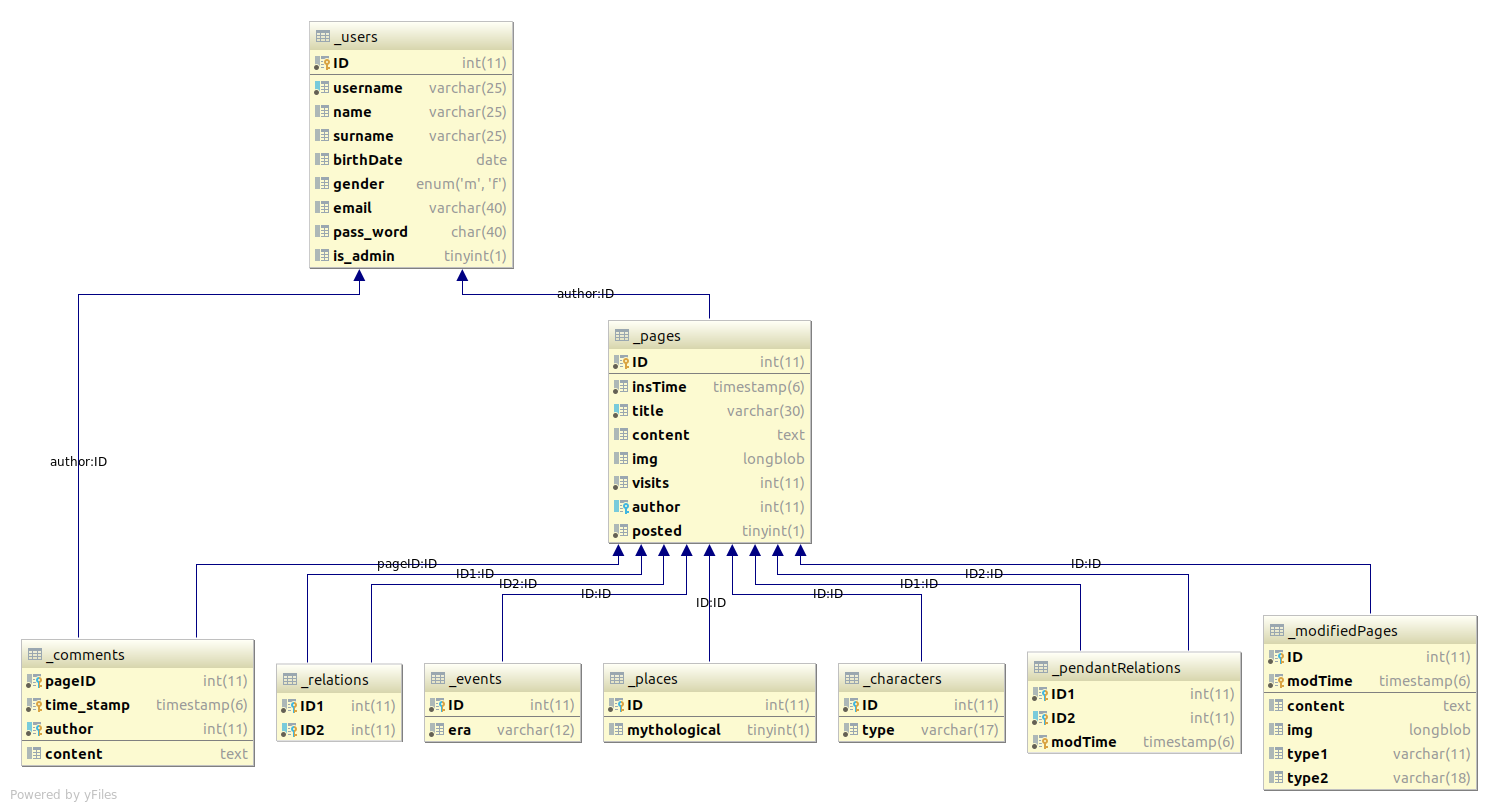
\includegraphics[width=14cm]{img/UML_database.png}
		\caption{UML Database}
	\end{center}
\end{figure}

\subsection{Accessibilità}
Per mantenere un alto livello di accessibilità abbiamo seguito lo standard WCAG 2.0.

\subsubsection{Separazione tra contenuto, presentazione e struttura}
Per migliorare l’accesso al sito agli utenti con differenti disabilità e ai motori di ricerca è stata mantenuta la separazione tra struttura, presentazione e comportamento.\\
La prima è stata sviluppata tramite documenti XHTML5, i quali richiamano i fogli di stile esterni CSS che implementano la presentazione e script esterni realizzati con JavaScript che formano il comportamento. Questi script sono stati implementati in modo da garantire una trasformazione elegante del sito, poiché se JavaScript è disabilitato il contenuto rimane comunque accessibile.\\
Tutto il codice redatto è stato scritto secondo le raccomandazioni W3C, accertando che fossero state rispettate tramite validazione. Si è evitato l’uso di tag e attributi deprecati.

\subsubsection{Navigazione} \label{subsection:navigazione}
Per quanto riguarda la navigazione è stata utilizzata la specifica WAI-ARIA prodotta da W3C, che definisce una serie di attributi HTML addizionali che possono essere applicati agli elementi per fornire maggior valore semantico e migliorare l'accessibilità dovunque sia necessario.

\paragraph{Breadcrumb} I breadcrumb sono una lista ordinata di pagine separate da front slash dove l'ultimo elemento, che è la pagina corrente, non ha link. A livello semantico è corretto che siano ordinati, infatti indicano l'ordine in cui un utente può raggiungere una determinata pagina.

\paragraph{Testo e link nascosti} Alcuni testi sono solo nascosti visivamente, ma vengono letti dagli screen reader. Per esempio "Ti trovi in:", che precede il breadcrumb, non viene visualizzato nella pagina, ma uno screen reader prima di leggere i breadcrumb, lo legge.\\
Alcuni link invece, vengono usati allo stesso modo del testo nascosto, ma la loro funzione è quella di saltare alcuni contenuti, ovvero di permettere agli utenti con gravi menomazioni visive di non leggere un determinato contenuto e passare direttamente al successivo.\\
Inoltre per migliorare la navigazione dello scroll, viene mostrato un pulsante in basso a destra dello schermo quando si scrolla verso il basso e, se un utente lo clicca, viene effettuato uno scroll verso l'alto fino all'inizio della pagina.

\paragraph{Attributi HTML} 
Le parole in lingue diverse da quella italiana sono state racchiuse all’interno di tag con l’attributo lang, per permettere una corretta lettura da parte degli screen reader. La pagina corrente nei breadcrumb ha l'attributo \textit{aria-current="page"} per indicare che quella è la pagina in cui l'utente si trova. Sempre nei breadcrumb, all'interno del tag nav compare \textit{aria-label="breadcrumb"} per indicare che il contenuto di quella navigazione indica la posizione dell'utente all'interno del sito.\\
Per indicare invece quali campi fossero obbligatori nella compilazione del form abbiamo usato \textit{aria-required}.
